% Options for packages loaded elsewhere
\PassOptionsToPackage{unicode}{hyperref}
\PassOptionsToPackage{hyphens}{url}
%
\documentclass[
]{article}
\usepackage{amsmath,amssymb}
\usepackage{iftex}
\ifPDFTeX
  \usepackage[T1]{fontenc}
  \usepackage[utf8]{inputenc}
  \usepackage{textcomp} % provide euro and other symbols
\else % if luatex or xetex
  \usepackage{unicode-math} % this also loads fontspec
  \defaultfontfeatures{Scale=MatchLowercase}
  \defaultfontfeatures[\rmfamily]{Ligatures=TeX,Scale=1}
\fi
\usepackage{lmodern}
\ifPDFTeX\else
  % xetex/luatex font selection
\fi
% Use upquote if available, for straight quotes in verbatim environments
\IfFileExists{upquote.sty}{\usepackage{upquote}}{}
\IfFileExists{microtype.sty}{% use microtype if available
  \usepackage[]{microtype}
  \UseMicrotypeSet[protrusion]{basicmath} % disable protrusion for tt fonts
}{}
\makeatletter
\@ifundefined{KOMAClassName}{% if non-KOMA class
  \IfFileExists{parskip.sty}{%
    \usepackage{parskip}
  }{% else
    \setlength{\parindent}{0pt}
    \setlength{\parskip}{6pt plus 2pt minus 1pt}}
}{% if KOMA class
  \KOMAoptions{parskip=half}}
\makeatother
\usepackage{xcolor}
\usepackage[margin=1in]{geometry}
\usepackage{graphicx}
\makeatletter
\def\maxwidth{\ifdim\Gin@nat@width>\linewidth\linewidth\else\Gin@nat@width\fi}
\def\maxheight{\ifdim\Gin@nat@height>\textheight\textheight\else\Gin@nat@height\fi}
\makeatother
% Scale images if necessary, so that they will not overflow the page
% margins by default, and it is still possible to overwrite the defaults
% using explicit options in \includegraphics[width, height, ...]{}
\setkeys{Gin}{width=\maxwidth,height=\maxheight,keepaspectratio}
% Set default figure placement to htbp
\makeatletter
\def\fps@figure{htbp}
\makeatother
\setlength{\emergencystretch}{3em} % prevent overfull lines
\providecommand{\tightlist}{%
  \setlength{\itemsep}{0pt}\setlength{\parskip}{0pt}}
\setcounter{secnumdepth}{-\maxdimen} % remove section numbering
\usepackage{titlesec}
\titleformat*{\section}{\normalfont\Large\bfseries\flushleft}
\titleformat*{\subsection}{\normalfont\large\bfseries\flushleft}
\titleformat*{\subsubsection}{\normalfont\normalsize\bfseries\flushleft}
\usepackage{amsmath}
\newcommand*{\defeq}{\mathrel{\vcenter{\baselineskip0.5ex \lineskiplimit0pt \hbox{\scriptsize.}\hbox{\scriptsize.}}}=}
\newcommand*{\eqdef}{=\mathrel{\vcenter{\baselineskip0.5ex \lineskiplimit0pt \hbox{\scriptsize.}\hbox{\scriptsize.}}}}
\ifLuaTeX
  \usepackage{selnolig}  % disable illegal ligatures
\fi
\usepackage{bookmark}
\IfFileExists{xurl.sty}{\usepackage{xurl}}{} % add URL line breaks if available
\urlstyle{same}
\hypersetup{
  pdftitle={Statistical Learning (5454) - Assignment 4},
  pdfauthor={Matthias Hochholzer, Lukas Pirnbacher, Anne Valder},
  hidelinks,
  pdfcreator={LaTeX via pandoc}}

\title{Statistical Learning (5454) - Assignment 4}
\author{Matthias Hochholzer, Lukas Pirnbacher, Anne Valder}
\date{Due: 2024-06-10}

\begin{document}
\maketitle

\section{Exercise 1}\label{exercise-1}

We generate data from the additive error model
\(Y = f(X_1,X_2) + \epsilon\), where \(f(X_1, X_2)\) is a sum of
sigmoids, i.e.
\[ f(X_1,X_2) = \sigma(a_1^\top X_1) + \sigma(a_2^\top X_2), \] with
\(a_1 = (3, 3)'\), \(a_2 = (3,-3)'\) and bivariate standard Gaussian
variables \(X_j\), \(j = 1, 2\). The variance of the independent
Gaussian error \(\epsilon\) is chosen such that the signal-to-noise
ratio as measured by the respective variances equals four. We generate a
training set of size 100 and a test sample of size 10,000.

We then fit neural networks with weight decay of 0.0005 and vary the
number of hidden units from 0 to 10. We record the average test error
\(E_{\text{Test}}(Y - \hat{f}(X_1,X_2))^2\) for each of 10 random
starting weights.

\begin{verbatim}
##    hidden_units mean_test_error sd_test_error
## 1             0       0.1569335   0.009344669
## 2             1       0.1805459   0.031403812
## 3             2       0.1531848   0.031377711
## 4             3       0.1357561   0.007124503
## 5             4       0.1354813   0.005213214
## 6             5       0.1347336   0.005268805
## 7             6       0.1309809   0.003254704
## 8             7       0.1306211   0.005273894
## 9             8       0.1320959   0.005098204
## 10            9       0.1333377   0.006381811
## 11           10       0.1320844   0.005652836
\end{verbatim}

Let us now visualize the results and interpret them.

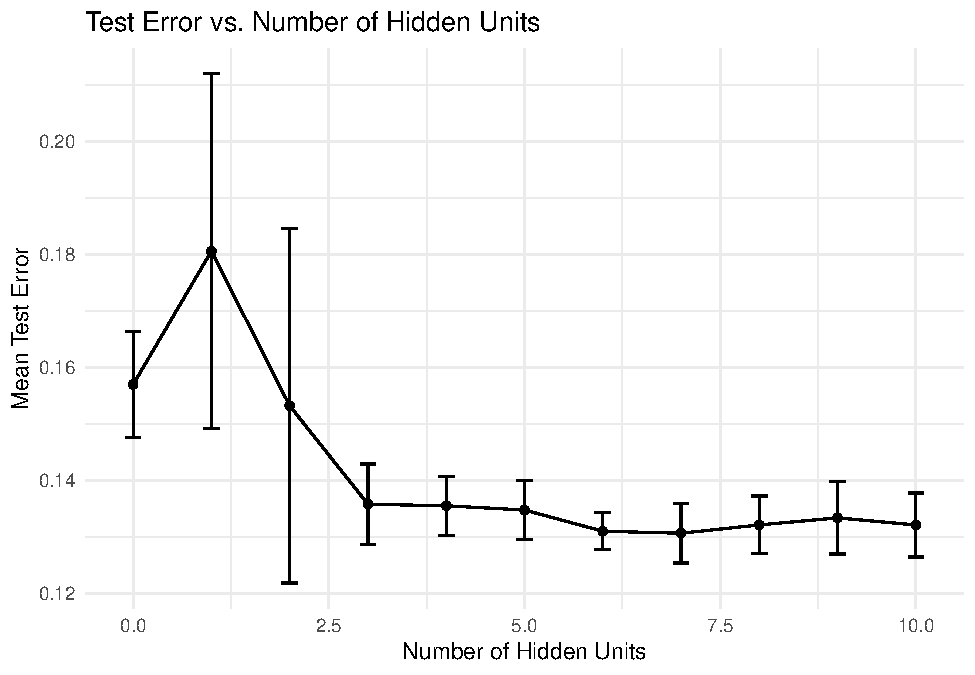
\includegraphics{A4_files/figure-latex/unnamed-chunk-5-1.pdf}

Out of all the models under consideration, the neural network with a
single hidden unit performs worst. It has the largest mean average test
error and also the largest variation in the average test error for
different random starting weights. Somewhat surprisingly, the linear
model, i.e.~the neural network with no hidden units, performs almost as
good as the neural network with two hidden units. While the mean average
test errors of these two models are similar, the average test error is
much less sensitive to different starting weights in case of the linear
model. All neural networks with 3 or more hidden units have a similar
performance, both in terms of the mean average test error and the
standard deviation of the average test error for different random
starting weights. Overall, we conclude that choosing a larger number of
hidden units and imposing shrinkage via weight decay appears to be
better than having too few hidden units in the first place.

\section{Exercise 2}\label{exercise-2}

The data sets \texttt{zip.train} and \texttt{zip.test} from package
\textbf{ElemStatLearn} contain information on the gray color values of
the pixels on a \(16 \times 16\) pixel image of hand-written digits. We
first visualize for each digit one randomly selected observation.

\begin{verbatim}
## [1] "digit  0  taken"
## [1] "digit  1  taken"
## [1] "digit  2  taken"
## [1] "digit  3  taken"
## [1] "digit  4  taken"
## [1] "digit  5  taken"
## [1] "digit  6  taken"
## [1] "digit  7  taken"
## [1] "digit  8  taken"
## [1] "digit  9  taken"
\end{verbatim}

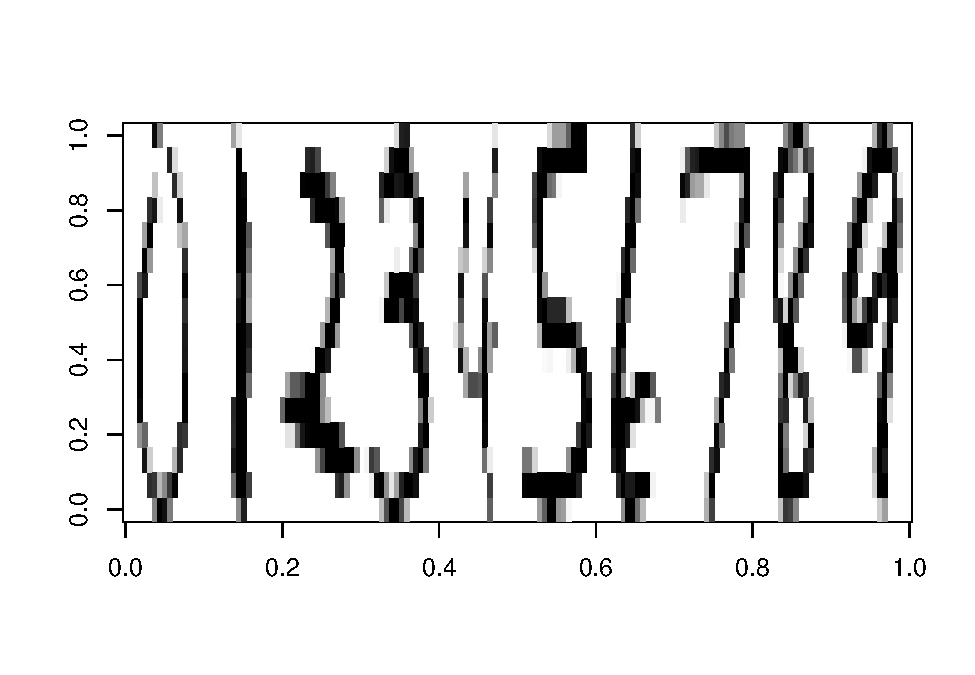
\includegraphics{A4_files/figure-latex/unnamed-chunk-6-1.pdf}

We now fit a multinomial logistic regression model to the training data
and evaluate it on the training and the test data. Before fitting the
model, however, we transform the data such that the regressors are
scaled on the unit interval.

\begin{verbatim}
## # weights:  2580 (2313 variable)
## initial  value 16788.147913 
## iter  10 value 2894.781800
## iter  20 value 1387.388893
## iter  30 value 805.767631
## iter  40 value 512.133103
## iter  50 value 274.070966
## iter  60 value 196.424106
## iter  70 value 148.210904
## iter  80 value 107.021614
## iter  90 value 72.525058
## iter 100 value 42.177330
## final  value 42.177330 
## stopped after 100 iterations
\end{verbatim}

We now determine the overall misclassification rate on the training and
the test data and the digit-specific misclassification rates on the test
data.

\begin{verbatim}
## [1] "misclassification rate (training data): 0.01%"
\end{verbatim}

\begin{verbatim}
## [1] "misclassification rate (test data): 12.11%"
\end{verbatim}

\begin{verbatim}
## [1] "digit-specific misclassification rates (test data):"
\end{verbatim}

\begin{verbatim}
##        0        1        2        3        4        5        6        7 
##   "3.9%"  "4.55%" "18.69%" "14.46%"    "21%" "16.88%"  "9.41%" "14.29%" 
##        8        9 
## "22.89%"  "6.78%"
\end{verbatim}

The misclassification rate on the training data is exceptionally low,
while the one on the test data is fairly high. The digits 8,4 and 2 are
particularly difficult to classify, whereas the model does a good job in
classifying 0,1, and 9.

The substantial discrepancy in performance between training and test
data suggests that overfitting may be an issue. Hence, we add a positive
weight decay of 0.05 when fitting the multinomial logistic regression
model in order to regularize it.

\begin{verbatim}
## # weights:  2580 (2313 variable)
## initial  value 16788.147913 
## iter  10 value 2909.202379
## iter  20 value 1423.990004
## iter  30 value 894.021900
## iter  40 value 614.653802
## iter  50 value 455.360357
## iter  60 value 417.148011
## iter  70 value 395.150898
## iter  80 value 384.312406
## iter  90 value 378.834838
## iter 100 value 376.137836
## final  value 376.137836 
## stopped after 100 iterations
\end{verbatim}

\begin{verbatim}
## [1] "misclassification rate (training data): 0.3%"
\end{verbatim}

\begin{verbatim}
## [1] "misclassification rate (test data): 9.32%"
\end{verbatim}

\begin{verbatim}
## [1] "digit-specific misclassification rates (test data):"
\end{verbatim}

\begin{verbatim}
##        0        1        2        3        4        5        6        7 
##   "3.9%"  "4.55%" "15.66%" "10.84%"  "13.5%" "13.75%"  "7.65%"  "10.2%" 
##        8        9 
## "15.06%"  "5.65%"
\end{verbatim}

Adding weight decay slightly increases the misclassification rate on the
training data, but reduces the misclassification rate on the test data.
The improved classification performance is particularly pronounced for
the ``difficult'\,' digits (8 and 4). Overall, adding a Ridge penalty to
the loss function, i.e.~adding the weight decay, improves the
out-of-sample performance of our model by mitigating the overfitting
problem.

\newpage

\section{Exercise 3}\label{exercise-3}

We continue using the data sets \texttt{zip.train} and \texttt{zip.test}
from package \textbf{ElemStatLearn}. However, we now only use a subset
of size 320 from \textit{zip.train}, with an equal number of
observations for each digit to fit a multinomial logistic regression
model and a neural network. We use the remaining observations from
\texttt{zip.train} and the test data to evaluate the fitted models.

Given the small sample size of the training data, overfitting is most
likely an issue. We therefore visualize the performance on the test data
in dependence of the training epochs when fitting the models.

\begin{verbatim}
## # weights:  2580 (2313 variable)
## initial  value 736.827230 
## iter  10 value 48.364930
## final  value 48.364930 
## stopped after 10 iterations
## # weights:  2580 (2313 variable)
## initial  value 736.827230 
## iter  10 value 48.364930
## iter  20 value 0.871059
## final  value 0.871059 
## stopped after 20 iterations
## # weights:  2580 (2313 variable)
## initial  value 736.827230 
## iter  10 value 48.364930
## iter  20 value 0.871059
## iter  30 value 0.071842
## final  value 0.071842 
## stopped after 30 iterations
## # weights:  2580 (2313 variable)
## initial  value 736.827230 
## iter  10 value 48.364930
## iter  20 value 0.871059
## iter  30 value 0.071842
## iter  40 value 0.024620
## iter  50 value 0.012972
## final  value 0.012972 
## stopped after 50 iterations
## # weights:  2580 (2313 variable)
## initial  value 736.827230 
## iter  10 value 48.364930
## iter  20 value 0.871059
## iter  30 value 0.071842
## iter  40 value 0.024620
## iter  50 value 0.012972
## iter  60 value 0.006339
## iter  70 value 0.003518
## iter  80 value 0.002358
## iter  90 value 0.001610
## iter 100 value 0.000943
## final  value 0.000943 
## stopped after 100 iterations
## # weights:  2580 (2313 variable)
## initial  value 736.827230 
## iter  10 value 48.364930
## iter  20 value 0.871059
## iter  30 value 0.071842
## iter  40 value 0.024620
## iter  50 value 0.012972
## iter  60 value 0.006339
## iter  70 value 0.003518
## iter  80 value 0.002358
## iter  90 value 0.001610
## iter 100 value 0.000943
## iter 110 value 0.000645
## iter 120 value 0.000491
## iter 130 value 0.000251
## iter 140 value 0.000245
## iter 150 value 0.000148
## final  value 0.000148 
## stopped after 150 iterations
## # weights:  2580 (2313 variable)
## initial  value 736.827230 
## iter  10 value 48.364930
## iter  20 value 0.871059
## iter  30 value 0.071842
## iter  40 value 0.024620
## iter  50 value 0.012972
## iter  60 value 0.006339
## iter  70 value 0.003518
## iter  80 value 0.002358
## iter  90 value 0.001610
## iter 100 value 0.000943
## iter 110 value 0.000645
## iter 120 value 0.000491
## iter 130 value 0.000251
## iter 140 value 0.000245
## iter 150 value 0.000148
## final  value 0.000097 
## converged
\end{verbatim}

\begin{verbatim}
## # weights:  3905
## initial  value 1663.464935 
## iter  10 value 79.681992
## final  value 79.681992 
## stopped after 10 iterations
## # weights:  3905
## initial  value 1672.904167 
## iter  10 value 72.661942
## iter  20 value 2.169041
## final  value 2.169041 
## stopped after 20 iterations
## # weights:  3905
## initial  value 1718.087019 
## iter  10 value 26.083447
## iter  20 value 0.310144
## iter  30 value 0.027409
## final  value 0.027409 
## stopped after 30 iterations
## # weights:  3905
## initial  value 1414.276942 
## iter  10 value 49.144805
## iter  20 value 0.711485
## iter  30 value 0.040968
## iter  40 value 0.012149
## iter  50 value 0.005050
## final  value 0.005050 
## stopped after 50 iterations
## # weights:  3905
## initial  value 1423.970760 
## iter  10 value 51.484734
## iter  20 value 1.462150
## iter  30 value 0.075633
## iter  40 value 0.017703
## iter  50 value 0.007656
## iter  60 value 0.003753
## iter  70 value 0.001567
## iter  80 value 0.001186
## iter  90 value 0.000469
## iter 100 value 0.000376
## final  value 0.000376 
## stopped after 100 iterations
## # weights:  3905
## initial  value 1716.030320 
## iter  10 value 53.207437
## iter  20 value 0.907040
## iter  30 value 0.056523
## iter  40 value 0.014348
## iter  50 value 0.005803
## iter  60 value 0.003249
## iter  70 value 0.001491
## iter  80 value 0.001056
## iter  90 value 0.000716
## iter 100 value 0.000387
## iter 110 value 0.000318
## iter 120 value 0.000176
## iter 130 value 0.000171
## final  value 0.000079 
## converged
## # weights:  3905
## initial  value 1945.337703 
## iter  10 value 93.956697
## iter  20 value 0.499032
## iter  30 value 0.065199
## iter  40 value 0.019139
## iter  50 value 0.007662
## iter  60 value 0.003780
## iter  70 value 0.002467
## iter  80 value 0.001238
## iter  90 value 0.000932
## iter 100 value 0.000293
## iter 110 value 0.000255
## iter 120 value 0.000223
## final  value 0.000092 
## converged
\end{verbatim}

\begin{verbatim}
## # weights:  5240
## initial  value 1733.045132 
## iter  10 value 34.775126
## final  value 34.775126 
## stopped after 10 iterations
## # weights:  5240
## initial  value 1775.725557 
## iter  10 value 48.130639
## iter  20 value 0.940412
## final  value 0.940412 
## stopped after 20 iterations
## # weights:  5240
## initial  value 2019.009483 
## iter  10 value 65.782554
## iter  20 value 0.447219
## iter  30 value 0.035726
## final  value 0.035726 
## stopped after 30 iterations
## # weights:  5240
## initial  value 1830.764123 
## iter  10 value 109.463346
## iter  20 value 0.604526
## iter  30 value 0.034259
## iter  40 value 0.007428
## iter  50 value 0.003200
## final  value 0.003200 
## stopped after 50 iterations
## # weights:  5240
## initial  value 1862.966329 
## iter  10 value 112.738462
## iter  20 value 1.364118
## iter  30 value 0.054795
## iter  40 value 0.010239
## iter  50 value 0.003593
## iter  60 value 0.001317
## iter  70 value 0.000752
## iter  80 value 0.000446
## iter  90 value 0.000247
## iter 100 value 0.000179
## final  value 0.000179 
## stopped after 100 iterations
## # weights:  5240
## initial  value 2257.881719 
## iter  10 value 138.424472
## iter  20 value 2.937467
## iter  30 value 0.086749
## iter  40 value 0.016862
## iter  50 value 0.004691
## iter  60 value 0.002354
## iter  70 value 0.001360
## iter  80 value 0.000739
## iter  90 value 0.000341
## iter 100 value 0.000231
## final  value 0.000094 
## converged
## # weights:  5240
## initial  value 1815.038186 
## iter  10 value 71.281739
## iter  20 value 0.655870
## iter  30 value 0.048885
## iter  40 value 0.011945
## iter  50 value 0.004802
## iter  60 value 0.002787
## iter  70 value 0.001407
## iter  80 value 0.000837
## iter  90 value 0.000416
## iter 100 value 0.000232
## iter 110 value 0.000164
## iter 120 value 0.000146
## final  value 0.000099 
## converged
\end{verbatim}

\begin{verbatim}
## # weights:  7910
## initial  value 1881.948733 
## iter  10 value 109.088936
## final  value 109.088936 
## stopped after 10 iterations
## # weights:  7910
## initial  value 1452.629520 
## iter  10 value 18.532800
## iter  20 value 0.301964
## final  value 0.301964 
## stopped after 20 iterations
## # weights:  7910
## initial  value 1707.344006 
## iter  10 value 55.575636
## iter  20 value 0.553530
## iter  30 value 0.039971
## final  value 0.039971 
## stopped after 30 iterations
## # weights:  7910
## initial  value 1663.993040 
## iter  10 value 61.140362
## iter  20 value 1.455502
## iter  30 value 0.049836
## iter  40 value 0.008999
## iter  50 value 0.003133
## final  value 0.003133 
## stopped after 50 iterations
## # weights:  7910
## initial  value 1577.776309 
## iter  10 value 19.437617
## iter  20 value 0.447892
## iter  30 value 0.023991
## iter  40 value 0.005424
## iter  50 value 0.002308
## iter  60 value 0.001038
## iter  70 value 0.000399
## iter  80 value 0.000315
## iter  90 value 0.000161
## iter 100 value 0.000130
## final  value 0.000130 
## stopped after 100 iterations
## # weights:  7910
## initial  value 1367.205805 
## iter  10 value 79.214546
## iter  20 value 0.815774
## iter  30 value 0.030266
## iter  40 value 0.007252
## iter  50 value 0.003066
## iter  60 value 0.001554
## iter  70 value 0.000748
## iter  80 value 0.000539
## iter  90 value 0.000214
## iter 100 value 0.000168
## final  value 0.000092 
## converged
## # weights:  7910
## initial  value 1653.554576 
## iter  10 value 85.165965
## iter  20 value 3.621547
## iter  30 value 0.089329
## iter  40 value 0.005340
## iter  50 value 0.001577
## iter  60 value 0.000309
## iter  70 value 0.000187
## final  value 0.000096 
## converged
\end{verbatim}

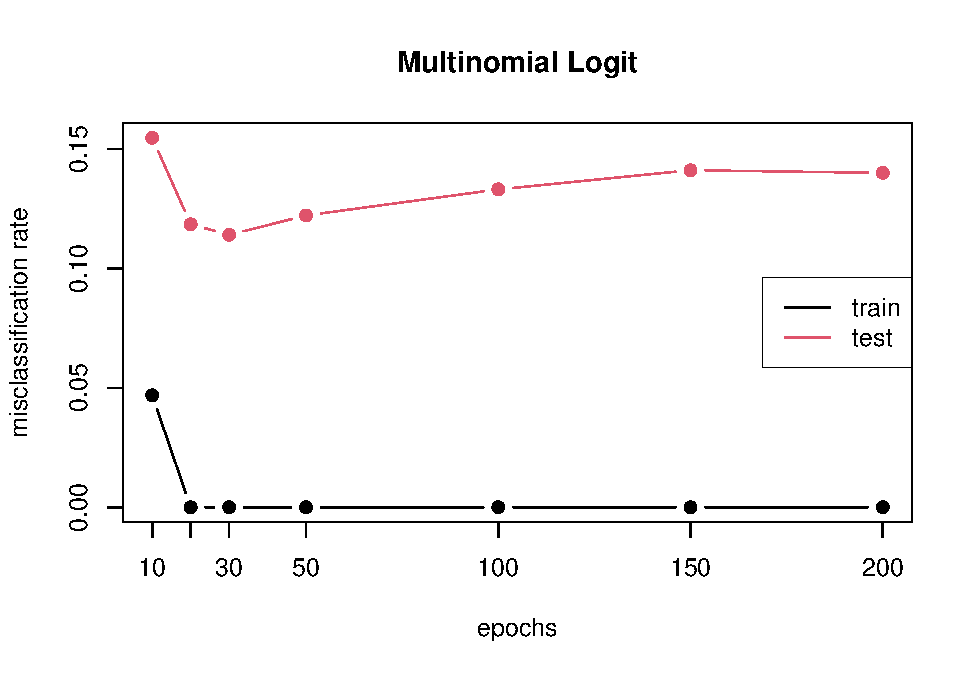
\includegraphics{A4_files/figure-latex/unnamed-chunk-10-1.pdf}
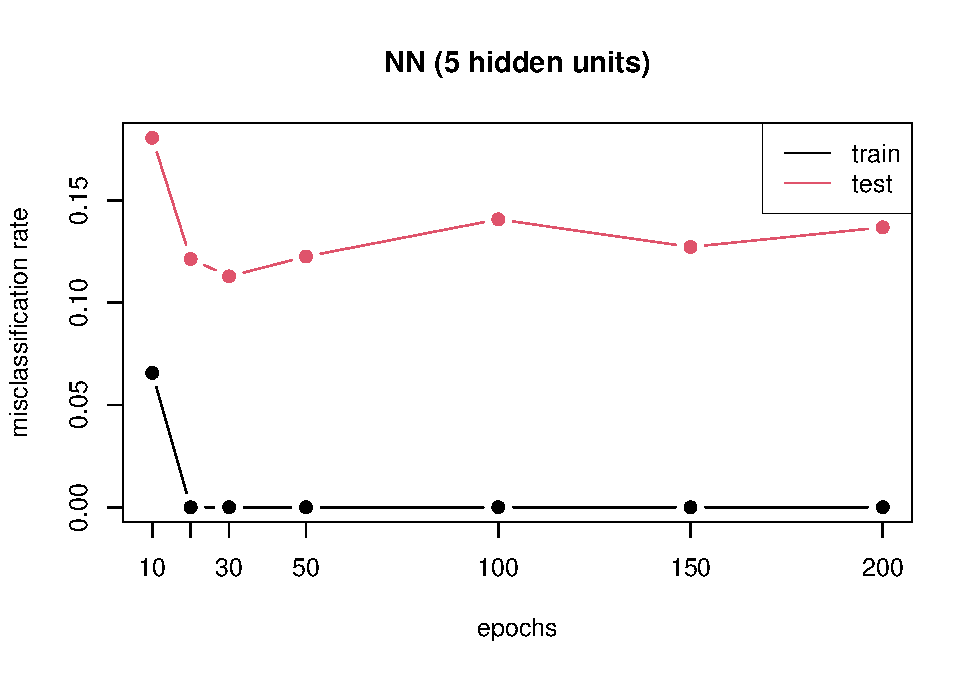
\includegraphics{A4_files/figure-latex/unnamed-chunk-10-2.pdf}
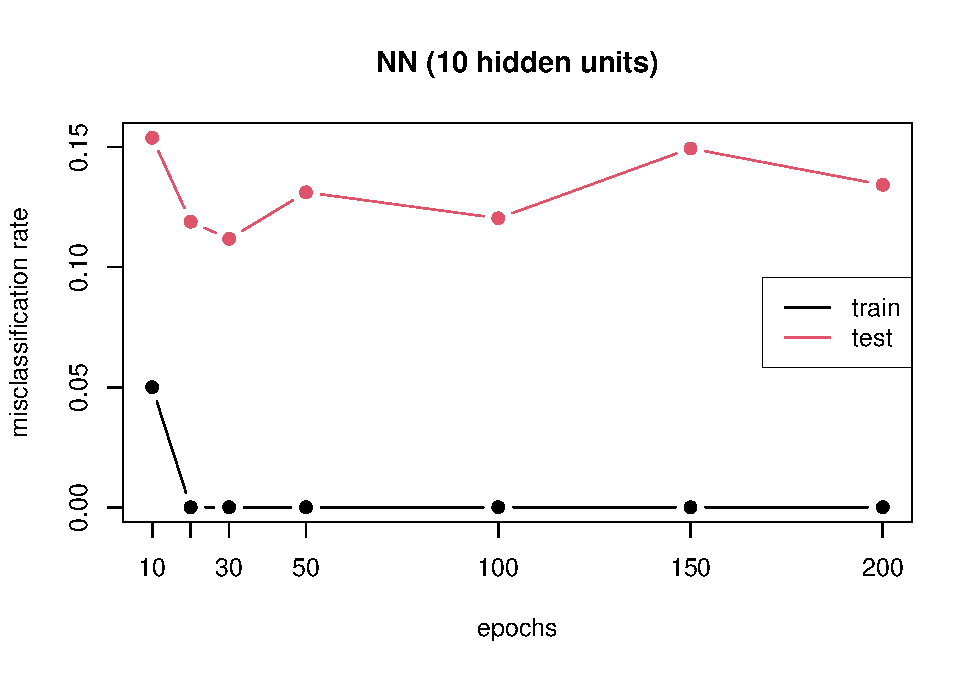
\includegraphics{A4_files/figure-latex/unnamed-chunk-10-3.pdf}
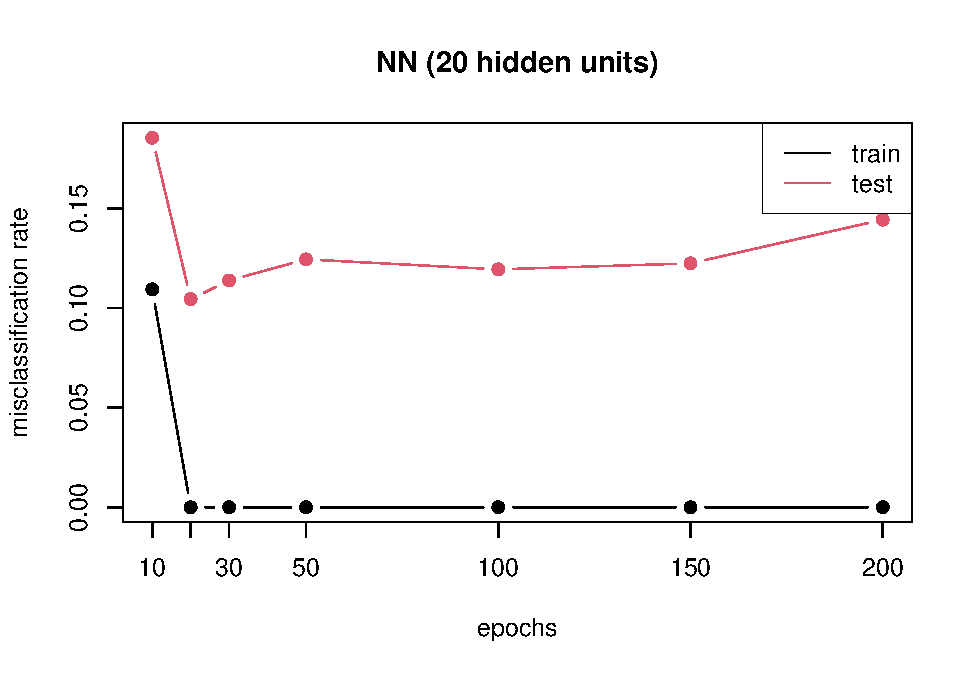
\includegraphics{A4_files/figure-latex/unnamed-chunk-10-4.pdf} The plots
are in line with our assumption that overfitting is an issue in this
exercise. For all models (multinomial logit, neural networks with 5, 10
and 20 hidden units) the misclassification rate on the test data
increases as the number of training epochs exceeds 30. Hence, in the
absence of a more explicit form of regularization (e.g.~a positive
weight decay) stopping the optimization routine early can be helpful to
improve out-of-sample performance.

\newpage

\section{Exercise 4}\label{exercise-4}

In the following we will estimate a predictive model for the
\texttt{Default} data from the \textbf{ISLR2} pacakge. We fit a neural
network using a single hidden layer with 10 units and dropout
regularization.

\begin{verbatim}
##   default student   balance    income
## 1      No      No  729.5265 44361.625
## 2      No     Yes  817.1804 12106.135
## 3      No      No 1073.5492 31767.139
## 4      No      No  529.2506 35704.494
## 5      No      No  785.6559 38463.496
## 6      No     Yes  919.5885  7491.559
\end{verbatim}

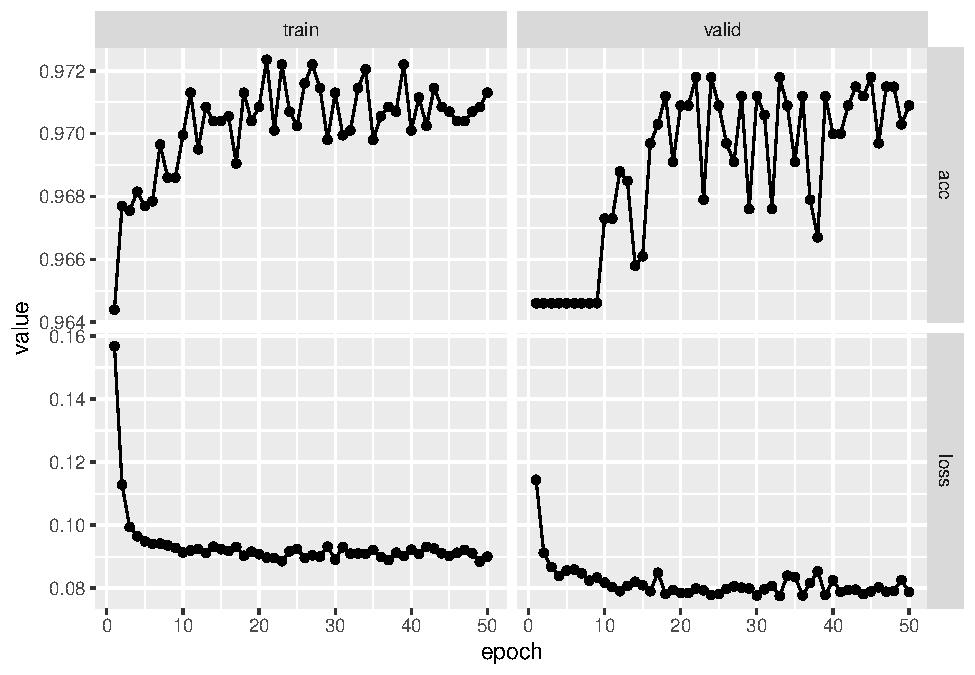
\includegraphics{A4_files/figure-latex/unnamed-chunk-11-1.pdf}

The linear logistic regression model performs very well on the test data
and has a classification accuracy of 97.18. Our neural network also
performs quite well and has a slightly lower accuracy of 97.09. Looking
at the plots above, we can see that the value of the loss function
decreases as the number of training epochs increases - for both the
training and the test data. Given that the loss function evaluated at
the test data does not increase as the number of epochs grows larger, we
find no evidence for overfitting. The classification performance
slightly improves as the number of training epochs increases. However,
it does not improve monotonically and the marginal gains are rather
negligible.

We now compare the classification performance of the two models more
closely.

\begin{verbatim}
## Type 'citation("pROC")' for a citation.
\end{verbatim}

\begin{verbatim}
## 
## Attaching package: 'pROC'
\end{verbatim}

\begin{verbatim}
## The following objects are masked from 'package:stats':
## 
##     cov, smooth, var
\end{verbatim}

\begin{verbatim}
## Setting levels: control = 0, case = 1
\end{verbatim}

\begin{verbatim}
## Setting direction: controls < cases
\end{verbatim}

\begin{verbatim}
## Setting levels: control = 0, case = 1
\end{verbatim}

\begin{verbatim}
## Setting direction: controls < cases
\end{verbatim}

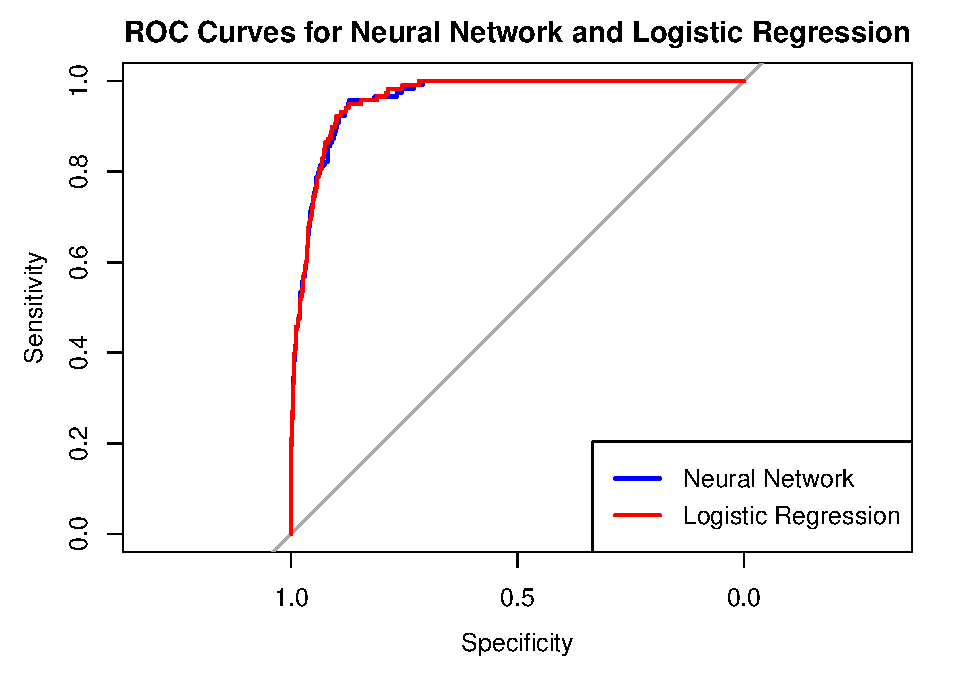
\includegraphics{A4_files/figure-latex/unnamed-chunk-12-1.pdf}

\begin{verbatim}
## AUC for Neural Network: 0.9611066
\end{verbatim}

\begin{verbatim}
## AUC for Logistic Regression: 0.9622321
\end{verbatim}

\begin{verbatim}
## Confusion Matrix and Statistics
## 
##           Reference
## Prediction    0    1
##          0 3212   94
##          1    3   24
##                                           
##                Accuracy : 0.9709          
##                  95% CI : (0.9646, 0.9763)
##     No Information Rate : 0.9646          
##     P-Value [Acc > NIR] : 0.02474         
##                                           
##                   Kappa : 0.3221          
##                                           
##  Mcnemar's Test P-Value : < 2e-16         
##                                           
##             Sensitivity : 0.9991          
##             Specificity : 0.2034          
##          Pos Pred Value : 0.9716          
##          Neg Pred Value : 0.8889          
##              Prevalence : 0.9646          
##          Detection Rate : 0.9637          
##    Detection Prevalence : 0.9919          
##       Balanced Accuracy : 0.6012          
##                                           
##        'Positive' Class : 0               
## 
\end{verbatim}

\begin{verbatim}
## Confusion Matrix and Statistics
## 
##           Reference
## Prediction    0    1
##          0 3202   81
##          1   13   37
##                                           
##                Accuracy : 0.9718          
##                  95% CI : (0.9656, 0.9772)
##     No Information Rate : 0.9646          
##     P-Value [Acc > NIR] : 0.01177         
##                                           
##                   Kappa : 0.4284          
##                                           
##  Mcnemar's Test P-Value : 4.829e-12       
##                                           
##             Sensitivity : 0.9960          
##             Specificity : 0.3136          
##          Pos Pred Value : 0.9753          
##          Neg Pred Value : 0.7400          
##              Prevalence : 0.9646          
##          Detection Rate : 0.9607          
##    Detection Prevalence : 0.9850          
##       Balanced Accuracy : 0.6548          
##                                           
##        'Positive' Class : 0               
## 
\end{verbatim}

\newpage

\section{Exercise 5}\label{exercise-5}

Now we perform document classification on the \textit{IMDb} data set,
which is available as part of the \textbf{torchdatasets} package. We
limit the dictionary size to the 10,000 most frequently-used words and
tokens. Again, we use James et al.~(2021, Chapter 10). We begin by
loading the data and creating a imdb\_tain and imdb\_test object. Each
element of imdb\_train is a vector of numbers between 1 and 10000 (the
document), referring to the words found in the dictionary. Next we write
a function to one-hot encode each document in a list of documents, and
return a binary matrix in sparse-matrix format. To construct the sparse
matrix, one supplies just the entries that are nonzero. In the last line
we call the function sparseMatrix() and supply the row indices
corresponding to each document and the column indices corresponding to
the words in each document, since we omit the values they are taken to
be all ones. Words that appear more than once in any given document
still get recorded as a one.

Consider the effects of varying the dictionary size. Try the values 500,
1000, 3000, 5000, and 10,000, and compare the results.

\end{document}
